%___________________________________________
% 1) Função seno
%___________________________________________

\begin{figure}[H]
  \centering
  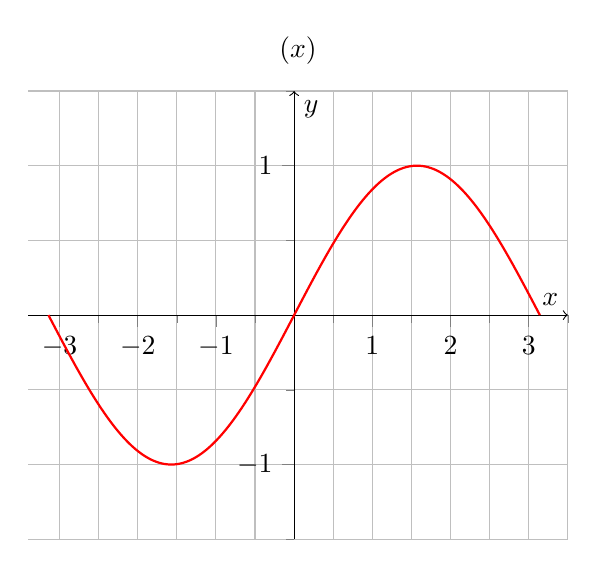
\begin{tikzpicture}
    \begin{axis}[
      xmin=-3.4, xmax=3.5,
      ymin=-1.5, ymax=1.5,
      axis x line=middle, 
      axis y line=middle,
      axis line style={->},
      tick align=outside,
      grid=both,
      minor tick num=1,
      xlabel={$x$},
      ylabel={$y$},
      title={$\sen(x)$}
    ]
      \addplot[red, thick, domain=-pi:pi, samples=200] {sin(deg(x))}; 
    \end{axis}
  \end{tikzpicture}
  \caption{Gráfico da função $\sen(x)$.}
\end{figure}
